% -------------------------------------------------------------------------------------------------
% CSI backbones: THAT (src/models/bce_that.py) and THATV (src/models/that_variance.py).
%
% Standalone TikZ diagram: compile with
%     pdflatex that_backbone_architecture.tex
% (or latexmk -pdf). Only the standard TikZ libraries are used, so any TeX Live/MiKTeX works.
%
% Two panels. Top: plain THAT, the single-vector encoder shared by every CSI model. Bottom: THATV,
% THAT plus three localization branches (temporal statistics, kept tokens, attention pooling), each
% independently switchable through preset["nn"]["backbone"] = "thatv[-nostats][,notokens][,nopool]".
%
% Shapes are (batch, time, feature) = (B, T, F). Both streams pool time with AvgPool1d(k20,s20), so
% the pooled length is N = T/20; WiMANS CSI is F = 3x3x30 = 270 and T = preset["data"]["length"] = 3000
% (H-WILD uses window 400). Head width D = embedding_dim (100, DensityMapNet) or d_embedding (64, AMAR).
% -------------------------------------------------------------------------------------------------
\documentclass[tikz,border=8pt]{standalone}
\usepackage[T1]{fontenc}
\usetikzlibrary{arrows.meta, positioning, fit, backgrounds, calc, shapes.geometric}

\definecolor{enc}{HTML}{2C7FB8}
\definecolor{head}{HTML}{D95F0E}
\definecolor{aux}{HTML}{756BB1}
\definecolor{keep}{HTML}{31A354}

\begin{document}
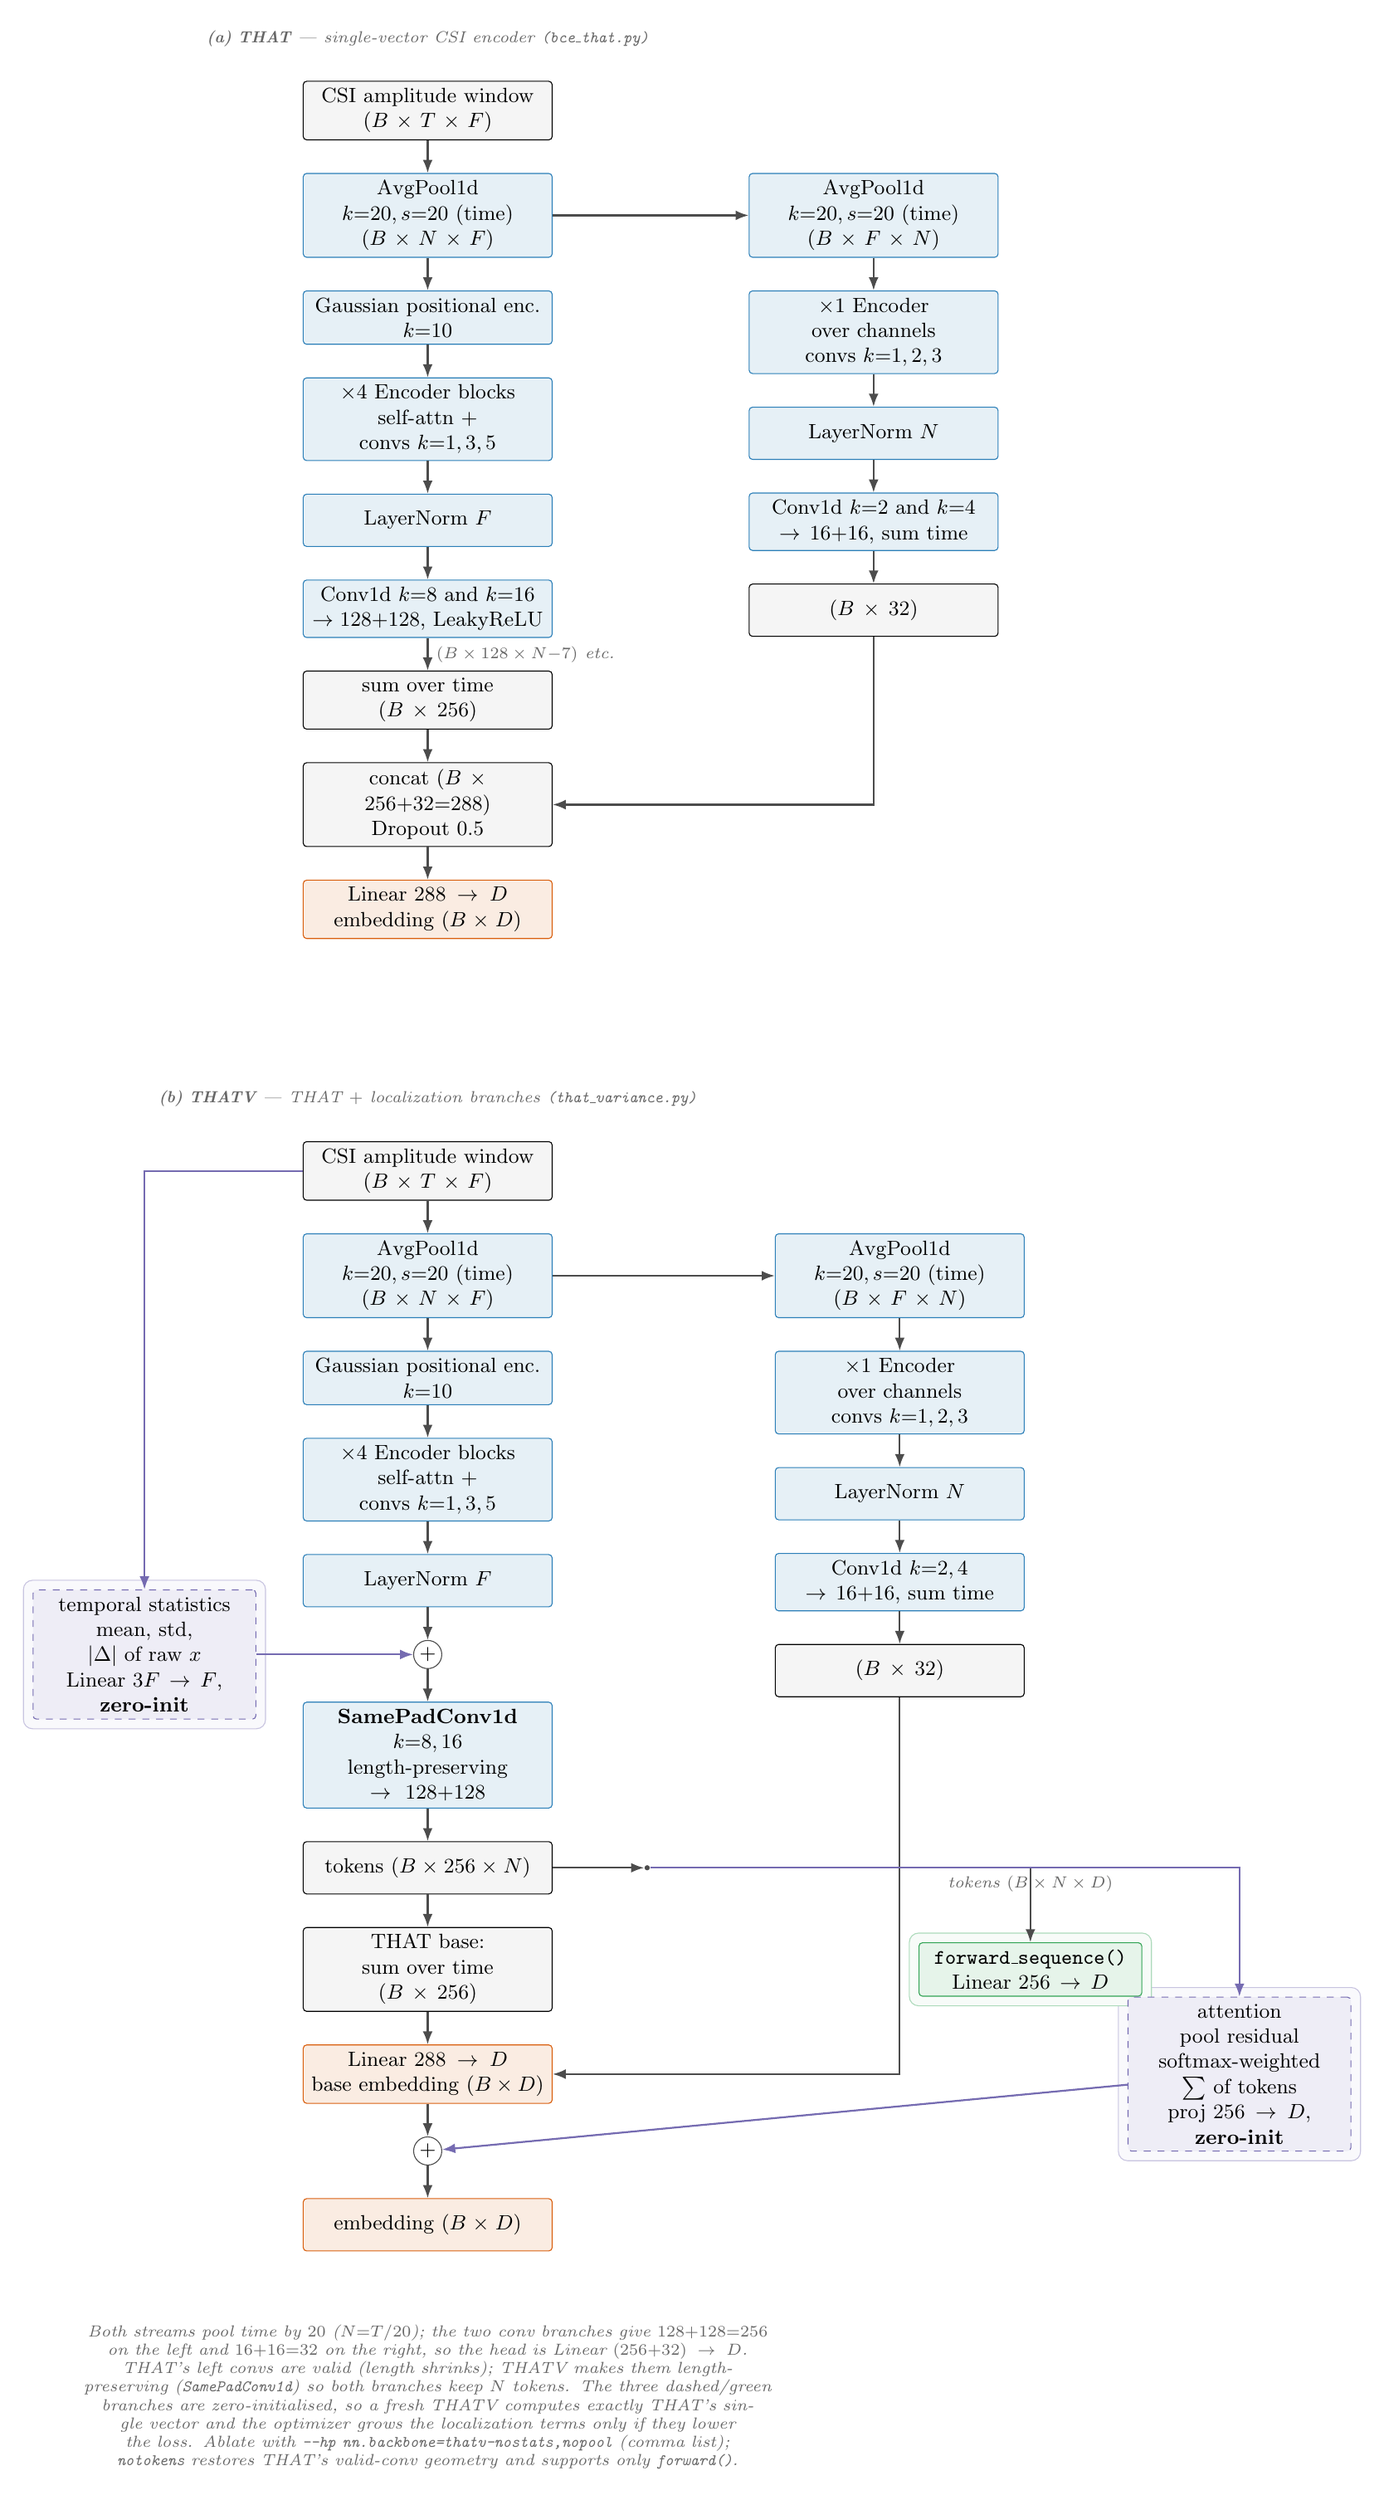
\begin{tikzpicture}[
    node distance = 5mm and 12mm,
    > = {Latex[length=2mm]},
    box/.style   = {draw, rounded corners=1.5pt, align=center, font=\small,
                    inner sep=3pt, minimum height=8mm, text width=36mm},
    tensor/.style = {box, fill=black!4},
    encbox/.style = {box, fill=enc!12,  draw=enc},
    headbox/.style= {box, fill=head!12, draw=head},
    auxbox/.style = {box, fill=aux!12,  draw=aux, dashed, text width=32mm},
    keepbox/.style= {box, fill=keep!12, draw=keep, text width=32mm},
    flow/.style   = {->, thick, draw=black!70},
    auxflow/.style= {->, thick, draw=aux},
    note/.style   = {font=\scriptsize\itshape, text=black!60},
    plus/.style   = {circle, draw=black!70, inner sep=1pt, font=\small, fill=white},
    dot/.style    = {circle, fill=black!70, inner sep=0.8pt},
]

% =================================================================================================
% ============================================ THAT ===============================================
% =================================================================================================
\node[note] at (0, 1.1) {\textbf{(a) THAT} --- single-vector CSI encoder \texttt{(bce\_that.py)}};

% ---------------------------------------- left stream (time-over-channel) -------------------------
\node[tensor]  (x)     at (0, 0) {CSI amplitude window\\$(B\times T\times F)$};
\node[encbox, below=of x]     (lpool) {AvgPool1d $k{=}20,s{=}20$ (time)\\$(B\times N\times F)$};
\node[encbox, below=of lpool] (lgauss){Gaussian positional enc.\\$k{=}10$};
\node[encbox, below=of lgauss](lenc)  {$\times4$ Encoder blocks\\self-attn $+$ convs $k{=}1,3,5$};
\node[encbox, below=of lenc]  (lnorm) {LayerNorm $F$};
\node[encbox, below=of lnorm] (lconv) {Conv1d $k{=}8$ and $k{=}16$\\$\to 128{+}128$, LeakyReLU};
\node[tensor, below=of lconv] (lsum)  {sum over time\\$(B\times 256)$};

% ---------------------------------------- right stream (channel-over-time) ------------------------
\node[encbox, right=30mm of lpool] (rpool) {AvgPool1d $k{=}20,s{=}20$ (time)\\$(B\times F\times N)$};
\node[encbox, below=of rpool] (renc)  {$\times1$ Encoder over channels\\convs $k{=}1,2,3$};
\node[encbox, below=of renc]  (rnorm) {LayerNorm $N$};
\node[encbox, below=of rnorm] (rconv) {Conv1d $k{=}2$ and $k{=}4$\\$\to 16{+}16$, sum time};
\node[tensor, below=of rconv] (rsum)  {$(B\times 32)$};

% ---------------------------------------------- head ---------------------------------------------
\node[tensor, below=of lsum] (cat) {concat $(B\times 256{+}32{=}288)$\\Dropout $0.5$};
\node[headbox, below=of cat] (out) {Linear $288\to D$\\embedding $(B\times D)$};

% --------------------------------------------- arrows --------------------------------------------
\draw[flow] (x) -- (lpool);
\draw[flow] (lpool) -- (lgauss);
\draw[flow] (lgauss) -- (lenc);
\draw[flow] (lenc) -- (lnorm);
\draw[flow] (lnorm) -- (lconv);
\draw[flow] (lconv) -- node[right, note] {$(B\times128\times N{-}7)$ etc.} (lsum);
\draw[flow] (lpool) -- (rpool);
\draw[flow] (rpool) -- (renc);
\draw[flow] (renc) -- (rnorm);
\draw[flow] (rnorm) -- (rconv);
\draw[flow] (rconv) -- (rsum);
\draw[flow] (lsum) -- (cat);
\draw[flow] (rsum) |- (cat);
\draw[flow] (cat) -- (out);

% =================================================================================================
% ============================================ THATV ==============================================
% =================================================================================================
\node[note] (vtitle) [below=22mm of out]
    {\textbf{(b) THATV} --- THAT $+$ localization branches \texttt{(that\_variance.py)}};

% ---------------------------------------- left stream (tokens kept) ------------------------------
\node[tensor]  (vx)     [below=4mm of vtitle] {CSI amplitude window\\$(B\times T\times F)$};
\node[encbox, below=of vx]     (vlpool) {AvgPool1d $k{=}20,s{=}20$ (time)\\$(B\times N\times F)$};
\node[encbox, below=of vlpool] (vlgauss){Gaussian positional enc.\\$k{=}10$};
\node[encbox, below=of vlgauss](vlenc)  {$\times4$ Encoder blocks\\self-attn $+$ convs $k{=}1,3,5$};
\node[encbox, below=of vlenc]  (vlnorm) {LayerNorm $F$};
\node[plus, below=of vlnorm]   (vadd)   {$+$};
\node[encbox, below=of vadd]   (vlconv) {\textbf{SamePadConv1d} $k{=}8,16$\\length-preserving $\to128{+}128$};
\node[tensor, below=of vlconv] (vlcat)  {tokens $(B\times 256\times N)$};

% ---------------------------------------- statistics branch (injected after LayerNorm) -----------
\node[auxbox, left=24mm of vadd] (vstat) {temporal statistics\\mean, std, $|\Delta|$ of raw $x$\\Linear $3F\to F$, \textbf{zero-init}};

% ---------------------------------------- right stream (unchanged from THAT) ----------------------
\node[encbox, right=34mm of vlpool] (vrpool) {AvgPool1d $k{=}20,s{=}20$ (time)\\$(B\times F\times N)$};
\node[encbox, below=of vrpool] (vrenc)  {$\times1$ Encoder over channels\\convs $k{=}1,2,3$};
\node[encbox, below=of vrenc]  (vrnorm) {LayerNorm $N$};
\node[encbox, below=of vrnorm] (vrconv) {Conv1d $k{=}2,4$\\$\to16{+}16$, sum time};
\node[tensor, below=of vrconv] (vrsum)  {$(B\times 32)$};

% ---------------------------------------- heads: forward() and forward_sequence() -----------------
\node[tensor, below=of vlcat] (vbase) {THAT base: sum over time\\$(B\times 256)$};
\node[headbox, below=of vbase] (vlin)  {Linear $288\to D$\\base embedding $(B\times D)$};
\node[dot, right=14mm of vlcat] (vtok) {};
\node[keepbox, right=56mm of vbase] (vseq) {\texttt{forward\_sequence()}\\Linear $256\to D$};
\node[auxbox, right=88mm of vlin] (vpool) {attention pool residual\\softmax-weighted $\sum$ of tokens\\proj $256\to D$, \textbf{zero-init}};
\node[plus, below=of vlin] (vaddp) {$+$};
\node[headbox, below=of vaddp] (vout) {embedding $(B\times D)$};

% --------------------------------------------- arrows --------------------------------------------
\draw[flow] (vx) -- (vlpool);
\draw[flow] (vlpool) -- (vlgauss);
\draw[flow] (vlgauss) -- (vlenc);
\draw[flow] (vlenc) -- (vlnorm);
\draw[flow] (vlnorm) -- (vadd);
\draw[flow] (vadd) -- (vlconv);
\draw[flow] (vlconv) -- (vlcat);
\draw[flow] (vlpool) -- (vrpool);
\draw[flow] (vrpool) -- (vrenc);
\draw[flow] (vrenc) -- (vrnorm);
\draw[flow] (vrnorm) -- (vrconv);
\draw[flow] (vrconv) -- (vrsum);
\draw[flow] (vlcat) -- (vbase);
\draw[flow] (vbase) -- (vlin);
\draw[flow] (vrsum) |- (vlin);
\draw[flow] (vlcat.east) -- (vtok);
\draw[flow] (vtok) -| (vseq.north) node[note, pos=0.72, above] {tokens $(B\times N\times D)$};
\draw[auxflow] (vtok) -| (vpool.north);
\draw[auxflow] (vx.west) -| (vstat.north);
\draw[auxflow] (vstat.east) -- (vadd.west);
\draw[auxflow] (vpool) -- (vaddp);
\draw[flow] (vlin) -- (vaddp);
\draw[flow] (vaddp) -- (vout);

% --------------------------------------------- groups --------------------------------------------
\begin{scope}[on background layer]
    \node[draw=aux!40,  fill=aux!4,  rounded corners, fit=(vstat), inner sep=4pt] {};
    \node[draw=aux!40,  fill=aux!4,  rounded corners, fit=(vpool), inner sep=4pt] {};
    \node[draw=keep!40, fill=keep!4, rounded corners, fit=(vseq), inner sep=4pt] {};
\end{scope}

% =================================================================================================
% ============================================ caption ============================================
% =================================================================================================
\node[note, below=10mm of vout, text width=110mm, align=center]
    {Both streams pool time by $20$ ($N{=}T/20$); the two conv branches give $128{+}128{=}256$ on the
     left and $16{+}16{=}32$ on the right, so the head is Linear $(256{+}32)\to D$. THAT's left convs are
     valid (length shrinks); THATV makes them length-preserving (\texttt{SamePadConv1d}) so both branches
     keep $N$ tokens. The three dashed/green branches are zero-initialised, so a fresh THATV computes
     exactly THAT's single vector and the optimizer grows the localization terms only if they lower the
     loss. Ablate with \texttt{--hp nn.backbone=thatv-nostats,nopool} (comma list); \texttt{notokens}
     restores THAT's valid-conv geometry and supports only \texttt{forward()}.};

\end{tikzpicture}
\end{document}
